% !TeX program = pdflatex
% =============================================================================
% Klasse 4fh: Reproduktion des an 4fh abgegebenen PDFs
% Vorlage: Klasse-fh/arbeitsblatt4-kondensatoren-teil1.pdf (24.08.2026, mit
% Loesungen), eingesetzt in der 4fh am 25.08.2026.
%
% Diese Fassung ist AELTER als arbeitsblatt4-kondensatoren.tex im Themenordner:
% Das Arbeitsblatt wurde am 27.08.2026 (zwischen der 4fh- und der
% 4cdeg-Lektion) umgebaut (Plenum-Boxen, Messen vor Definition, ungerahmtes
% Box-Layout). Hier steht deshalb der Stand vor dem Umbau: farbige Boxen,
% sechs Lernziele LZ1-LZ6, Definition C = Q/U direkt in der Theorie,
% Wassertankanalogie mit Fliesstext, Herleitung der Kondensatorformel nur im
% Aufgabenblatt (Teil 2c). Text aus dem 4fh-PDF rekonstruiert, Bildbreiten
% nach Augenmass.
% =============================================================================
\documentclass[addpoints,11pt,a4paper]{exam}

\usepackage[T1]{fontenc}
\usepackage[utf8]{inputenc}
\usepackage[ngerman]{babel}
\usepackage{lmodern}
\usepackage[a4paper,margin=2.2cm,headheight=14pt]{geometry}
\usepackage{amsmath}
\usepackage{siunitx}
\sisetup{per-mode=fraction,fraction-command=\frac}
\usepackage{array,booktabs,tabularx,multirow}
\usepackage{enumitem}
\usepackage{xcolor}
\usepackage{colortbl}
\usepackage{tikz}
\usepackage{physics}
\usepackage{circuitikz}
\usepackage[most]{tcolorbox}
\usepackage{lastpage}
\usepackage{graphicx}
% Bilder liegen im uebergeordneten Themenordner (nicht dupliziert).
\graphicspath{{../}}
\usepackage{hyperref}

\usetikzlibrary{arrows.meta,calc,angles,quotes}

\usepackage{setspace}
\usepackage{needspace}
\setlength{\parindent}{0pt}
\setlength{\parskip}{0.6em}
\setstretch{1.08}
\setlist[itemize]{itemsep=0.4em}

% -----------------------------
% Farben (Corporate-Farbschema Physik KFR)
% -----------------------------
\definecolor{titleblue}{HTML}{183A6B}
\definecolor{accentblue}{HTML}{2E6F9E}
\definecolor{lightblue}{HTML}{EAF4FB}
\definecolor{verylightblue}{HTML}{F7FBFE}
\definecolor{lightgray}{HTML}{F4F6F8}
\definecolor{darkgray}{HTML}{4A4A4A}
\definecolor{accentorange}{HTML}{D9720C}
\definecolor{accentpurple}{HTML}{7B2D8E}
\definecolor{theorygreen}{HTML}{2E7D4F}
\definecolor{lighttheorygreen}{HTML}{EAF7EF}
\definecolor{groupteal}{HTML}{1B7F72}
\definecolor{lightgroupteal}{HTML}{E8F5F3}
\definecolor{lightorange}{HTML}{FCEEE0}

\hypersetup{
  colorlinks=true,
  urlcolor=accentblue,
  linkcolor=accentblue,
  pdftitle={Arbeitsblatt 4: Kondensatoren},
  pdfauthor={Loris Keller}
}

\newcolumntype{Y}{>{\centering\arraybackslash}X}
\newcolumntype{P}[1]{>{\raggedright\arraybackslash}p{#1}}

% -----------------------------
% Boxen (farbiges Layout, Stand 4fh vor der Umstellung vom 31.08.2026)
% -----------------------------
\tcbset{before skip=10pt, after skip=10pt}
\newtcolorbox{titlebox}{
  enhanced,
  colback=titleblue,
  colframe=titleblue,
  boxrule=0pt,
  arc=3mm,
  left=3mm,right=3mm,top=3mm,bottom=3mm
}

\newlength{\aufgabenindent}
\settowidth{\aufgabenindent}{10.\hskip\labelsep}

\newtcolorbox{infobox}{
  enhanced,
  breakable,
  colback=lightblue,
  colframe=accentblue,
  boxrule=0.7pt,
  arc=2mm,
  left=6mm,right=6mm,top=3.5mm,bottom=3.5mm
}

\newtcolorbox{theoriebox}[1][Theorie]{
  enhanced,
  breakable,
  colback=lighttheorygreen,
  colframe=theorygreen,
  title={#1},
  fonttitle=\bfseries,
  boxrule=0.7pt,
  arc=2mm,
  left=6mm,right=6mm,top=3.5mm,bottom=3.5mm
}

\newtcolorbox{beispielbox}[1][Beispiel]{
  enhanced,
  breakable,
  colback=verylightblue,
  colframe=accentblue,
  title={#1},
  fonttitle=\bfseries,
  boxrule=0.7pt,
  arc=2mm,
  left=5mm,right=5mm,top=2mm,bottom=2mm
}

\newtcolorbox{groupbox}[1][Gruppenarbeit]{
  enhanced,
  breakable,
  colback=lightgroupteal,
  colframe=groupteal,
  title={#1},
  fonttitle=\bfseries,
  boxrule=0.7pt,
  arc=2mm,
  enlarge left by=-\aufgabenindent,
  width=\textwidth,
  left=6mm,right=6mm,top=3.5mm,bottom=3.5mm
}

\newtcolorbox{hinweisbox}[1][Hinweis]{
  enhanced,
  breakable,
  colback=lightorange,
  colframe=accentorange,
  title={#1},
  fonttitle=\bfseries,
  boxrule=0.7pt,
  arc=2mm,
  left=5mm,right=5mm,top=2mm,bottom=2mm
}

\newtcolorbox{answerbox}{
  breakable,
  colback=white,
  colframe=gray!55,
  boxrule=0.5pt,
  arc=1.5mm,
  left=2mm,right=2mm,top=2mm,bottom=2mm
}

% --- Lösungen ein-/ausblenden -----------------------------------------------
% Schuelerversion (Standard):  pdflatex <name>.tex
% Loesungsversion:             pdflatex -jobname=<name>_Loesung "\def\MitLoesung{}\input{<name>}"
\ifdefined\MitLoesung\printanswers\else\noprintanswers\fi

\pointformat{}
\renewcommand{\solutiontitle}{\noindent\color{titleblue}\textbf{Lösung:}\enspace}

\pagestyle{headandfoot}
\cfoot{\textcolor{darkgray}{Seite \thepage\ von \pageref{LastPage}}}

\newcommand{\Kopfzeile}[4]{%
  \begin{titlebox}
    {\color{white}\sffamily\bfseries\Large #4}
  \end{titlebox}
  \vspace{0.5em}
  \noindent\textbf{Klasse:}~#1 \hfill \textbf{Datum:}~#2 \hfill \textbf{Thema:}~#3
    \hfill \textbf{Lehrperson:}~Loris Keller
  \vspace{0.8em}
  \lhead{\textcolor{darkgray}{#3}}
  \rhead{\textcolor{darkgray}{#4}}
}

\newlength{\antwortraumlen}
\newcommand{\Antwortraum}[1]{%
  \pgfmathsetlength{\antwortraumlen}{#1*2.5cm}%
  \begin{answerbox}
    \rule{0pt}{\antwortraumlen}%
  \end{answerbox}%
}

% Werte für Kopfzeile zentral setzen (wie im 4fh-PDF)
\newcommand{\Klasse}{4fh / 4cdeg (SP4)}
\newcommand{\Datum}{25.08.2026 (4fh) / 28.08.2026 (4cdeg)}
\newcommand{\Thema}{Kondensatoren}
\newcommand{\ArbeitsblattTitel}{Arbeitsblatt 4: Kondensatoren}

\begin{document}

\Kopfzeile{\Klasse}{\Datum}{\Thema}{\ArbeitsblattTitel}

% =============================================================================
% Lernziele
% =============================================================================
\begin{infobox}
\textbf{Lernziele}\\
Am Ende dieser Doppellektion kann ich \dots
\begin{itemize}[leftmargin=1.2cm,itemsep=0.3em]
  \item die Kapazität $C=Q/U$ als definierende Grösse eines Kondensators
  nennen (Einheit Farad), bevor eine Analogie zur Veranschaulichung
  herangezogen wird. (LZ1)
  \item erklären, was ein Kondensator ist und wozu er in einer Schaltung
  gebraucht wird (Ladungs-/Energiespeicher), gestützt auf die
  Wassertankanalogie als Veranschaulichung der bereits definierten
  Kapazität. (LZ2)
  \item aus eigenen Messdaten den Zusammenhang zwischen $Q$ und $U$
  untersuchen und daraus die Kapazität des verwendeten Kondensators
  bestimmen. (LZ3)
  \item durch eigene Messungen und eine algebraische Herleitung
  herausfinden, wie Plattenfläche $A$ und Plattenabstand $d$ die Kapazität
  beeinflussen. (LZ4)
  \item für einen von der Spannungsquelle getrennten Kondensator
  vorhersagen und begründen, wie sich Ladung und Spannung bei einer
  Änderung der Plattengeometrie verhalten. (LZ5)
  \item erklären, was ein Dielektrikum ist, und herleiten, welchen Einfluss
  es auf die Kapazität eines Kondensators hat. (LZ6)
\end{itemize}
\end{infobox}

% =============================================================================
% Einleitung
% =============================================================================
\begin{beispielbox}[Einleitung: Wozu braucht man unterschiedliche Kapazitäten?]
\begin{center}
  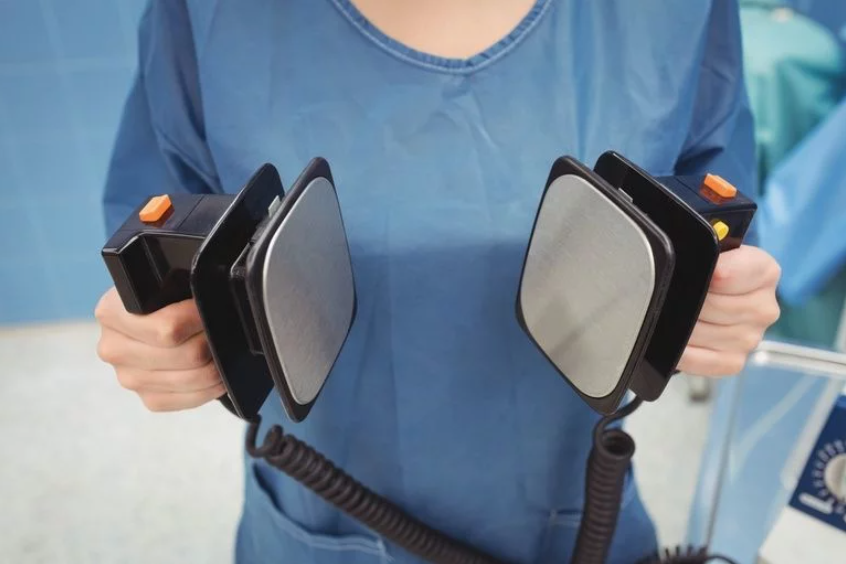
\includegraphics[width=4.5cm]{Bilder/defibrillator.png}
\end{center}

Die Kapazität $C$ legt fest, wie viel Ladung ein Kondensator bei einer
bestimmten Spannung speichern kann -- je nach Anwendung braucht man dafür
ganz unterschiedliche Werte.

\textbf{\emph{Hohe Kapazität}} braucht es, wenn viel Energie gespeichert
und dann sehr schnell wieder abgegeben werden soll: Ein
\textbf{\emph{Defibrillator}} lädt sich langsam auf, gibt die gespeicherte
Ladung dann aber innert Millisekunden als kräftigen Stromstoss ab.

\textbf{\emph{Tiefe Kapazität}} genügt dagegen, wenn nur eine winzige
Ladungsänderung erkannt werden muss: Der \textbf{\emph{Touchscreen}} Ihres
Smartphones misst an jedem Punkt eine kleine Kapazität und erkennt so, wo
Sie ihn berühren.
\end{beispielbox}

% =============================================================================
% Theorie 1: Der Kondensator und die Wassertankanalogie
% =============================================================================
\begin{theoriebox}[Der Kondensator und die Wassertankanalogie]
Ein \textbf{\emph{Kondensator}} besteht in seiner einfachsten Form, dem
\textbf{\emph{Plattenkondensator}}, aus zwei parallelen, leitenden Platten,
die sich nicht berühren. Zwischen den Platten befindet sich ein
elektrischer Isolator, das sogenannte \textbf{\emph{Dielektrikum}}
(zunächst einfach Luft). Legt man über die beiden Platten eine Spannung
an, fliessen Elektronen von der einen Platte weg und auf die andere: Die
eine Platte trägt am Ende die Ladung $+Q$, die andere $-Q$. Die
Gesamtladung bleibt also neutral. Gespeichert wird die \emph{getrennte}
Ladung.

\begin{center}
\begin{tikzpicture}[>=Latex,scale=2]
  \draw[very thick] (0,-1.5) -- (0,1.5);
  \draw[very thick] (2.6,-1.5) -- (2.6,1.5);
  \foreach \y in {-1.1,-0.55,0,0.55,1.1} {
    \node at (-0.2,\y) {$+$};
    \node at (2.8,\y) {$-$};
  }
  \foreach \y in {-0.9,-0.45,0,0.45,0.9} {
    \draw[->,accentblue] (0.15,\y) -- (2.45,\y);
  }
  \draw[<->] (0,-1.9) -- (2.6,-1.9) node[midway,below] {$d$};
  \node[accentblue] at (1.3,1.85) {$\vec{E}$};
\end{tikzpicture}
\hspace{1.2cm}
\begin{circuitikz}[scale=2.1]
  \draw (0,0) to[capacitor,l=$C$] (2,0);
\end{circuitikz}
\end{center}
{\scriptsize Links: Plattenkondensator im Querschnitt, mit homogenem
elektrischem Feld $\vec E$ zwischen den Platten. Rechts: Schaltzeichen für
einen Kondensator.}

Diese Fähigkeit, getrennte Ladung zu speichern, wird durch die
\textbf{\emph{Kapazität}} $C$ eines Kondensators beschrieben. Sie ist
definiert als das Verhältnis von gespeicherter Ladung $Q$ zur anliegenden
Spannung $U$:
\[
  \boxed{C := \frac{Q}{U}}, \qquad [C] = 1\,\frac{\text{C}}{\text{V}} = 1\ \text{Farad} = \SI{1}{\farad}.
\]
Je grösser $C$, desto mehr Ladung $Q$ kann der Kondensator bei gegebener
Spannung $U$ speichern.

In der Praxis sind Kapazitäten oft winzig. Deshalb wird meist nicht Farad
selbst, sondern eine kleinere Einheit mit vorangestelltem Präfix
angegeben:
\[
  \SI{1}{\pico\farad} = \SI{e-12}{\farad}, \quad
  \SI{1}{\nano\farad} = \SI{e-9}{\farad}, \quad
  \SI{1}{\micro\farad} = \SI{e-6}{\farad}, \quad
  \SI{1}{\milli\farad} = \SI{e-3}{\farad}.
\]
Ein Kondensator mit $C=\SI{100}{\pico\farad}$ hat also die Kapazität
$C=\SI{100e-12}{\farad}=\SI{1e-10}{\farad}$.

\begin{hinweisbox}[Achtung: Verwechslungsgefahr C und Coulomb]
Das Formelzeichen $C$ für die Kapazität hat nichts mit der Einheit
\textbf{\emph{Coulomb}} zu tun, die ebenfalls mit dem Buchstaben C
abgekürzt wird (\si{\coulomb}) und in der die Ladung $Q$ gemessen wird.
Steht irgendwo z.\,B. $Q=\SI{2}{\coulomb}$, ist damit die Ladungseinheit
gemeint, nicht die Kapazität. Die Kapazität selbst wird in Farad
angegeben.
\end{hinweisbox}

\textbf{Die Wassertankanalogie:} Die soeben definierte Kapazität lässt
sich gut mit einem Wassertank veranschaulichen.
\begin{center}
  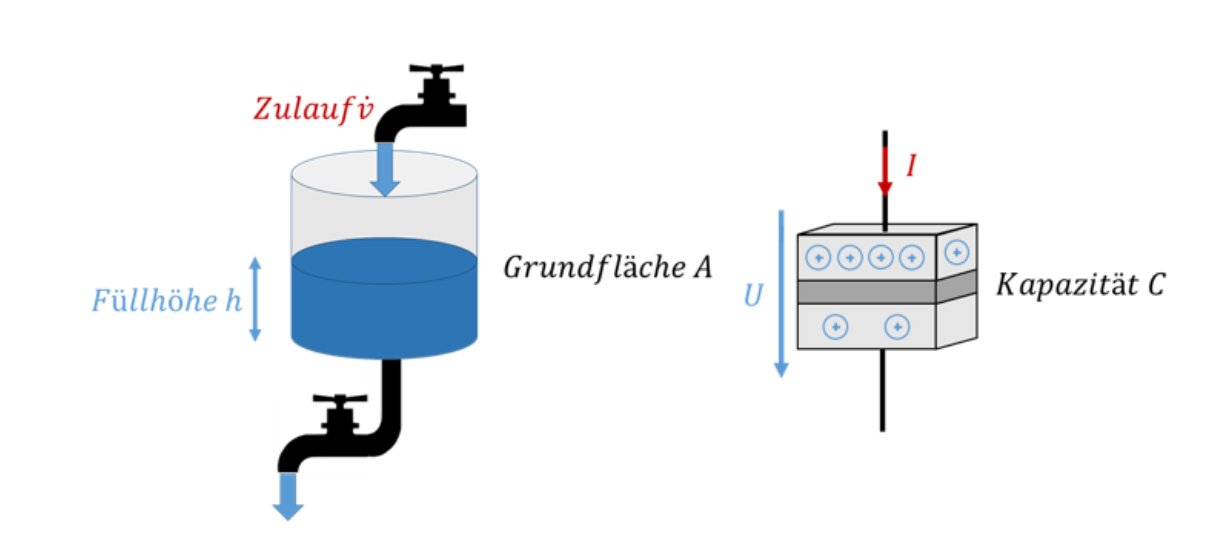
\includegraphics[width=11cm]{Bilder/wasserfass-vs-kondensator.png}
\end{center}
{\scriptsize Ein Wassertank als mechanische Analogie zu einem
Kondensator.}

Stellen Sie sich einen Wassertank mit Grundfläche $A_{\text{Tank}}$ vor,
der über eine Leitung mit Wasser gefüllt wird: Je grösser die Grundfläche,
desto weniger stark steigt der Füllstand $h$ pro zugeführter Wassermenge.
Welche Grösse des Kondensators sich dabei wie die Grundfläche verhält und
welche wie der Füllstand, finden Sie in der folgenden Sortieraufgabe
selbst heraus.

Die Analogie erklärt auch gleich, wozu das in der Einleitung gut ist
(Defibrillator): Reicht die Hauptleitung allein nicht aus, um einen
kurzfristig hohen Bedarf (\glqq Last\grqq{}) zu decken, lässt sich
zusätzlich ein Ventil zum Speicher öffnen. Der zuvor gefüllte Speicher
liefert dann für kurze Zeit zusätzliches Wasser, bis er sich leert.

\begin{center}
  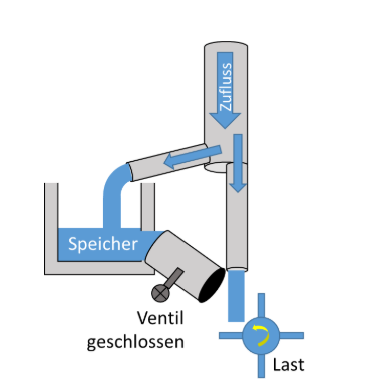
\includegraphics[width=5cm]{Bilder/wassertank_ventil_zu.png}
  \hspace{0.8cm}
  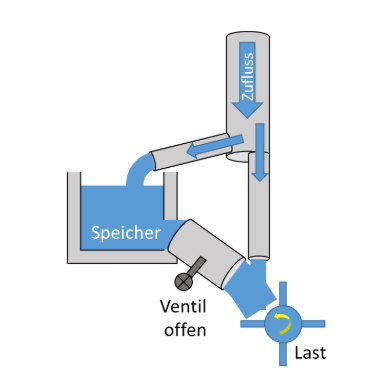
\includegraphics[width=5cm]{Bilder/wassertank_ventil_offen.png}
\end{center}
{\scriptsize Links: Ventil geschlossen, nur die Hauptleitung versorgt die
Last. Rechts: Ventil geöffnet, der Speicher liefert zusätzliches Wasser.}

Genauso ist es beim Kondensator: Reicht die Batterie allein nicht aus, um
kurzfristig sehr viel Strom zu liefern, liefert der zuvor aufgeladene
Kondensator für kurze Zeit zusätzliche Ladung, bis er entladen ist.
\end{theoriebox}

% =============================================================================
% Sortieraufgabe
% =============================================================================
\begin{questions}
\begin{groupbox}[Sortieraufgabe: Wassertank vs. Kondensator]
\question[5] Ordnen Sie auch hier zu zweit die Grössen des Wassertanks
(links) den entsprechenden Grössen des Kondensators (rechts) zu, indem Sie
sie mit dem Stift verbinden.

\begin{center}
\renewcommand{\arraystretch}{1.3}
\begin{tabular}{>{\raggedleft\arraybackslash}p{4.6cm}c@{\hspace{2.2cm}}cP{4.6cm}}
1. Grundfläche $A_{\text{Tank}}$ des Tanks & $\bullet$ & $\bullet$ & A. Ladung $Q$ \\
2. Füllstand $h$ (Wasserspiegelhöhe) & $\bullet$ & $\bullet$ & B. Kapazität $C$ \\
3. Wassermenge im Tank & $\bullet$ & $\bullet$ & C. Spannung $U$ \\
4. Maximales Volumen $V_{\max}=A_{\text{Tank}}\cdot h_{\max}$ & $\bullet$ & $\bullet$ & D. Lade-/Entladestrom \\
5. Zu-/Abfluss von Wasser & $\bullet$ & $\bullet$ & E. Maximale Ladung $Q_{\max}=C\cdot U_{\max}$ \\
\end{tabular}
\renewcommand{\arraystretch}{1}
\end{center}

\begin{solution}
1 passt zu B, 2 passt zu C, 3 passt zu A, 4 passt zu E, 5 passt zu D.
\end{solution}
\end{groupbox}
\end{questions}

% =============================================================================
% Theorie 2: Kapazität und Plattengeometrie
% =============================================================================
\begin{theoriebox}[Kapazität und Plattengeometrie: die bekannten Bausteine]
\textbf{Repetition:} Aus der Elektrostatik wissen Sie bereits, dass die
elektrische Feldstärke einer geladenen Platte
$E=\frac{Q}{2\varepsilon_0\cdot A}$ beträgt, und dass sich zwischen zwei
Platten eines Plattenkondensators die Feldstärke verdoppelt:
\[
  \boxed{E = \frac{Q}{\varepsilon_0\cdot A}} \qquad \text{(zwischen den Platten, Randeffekte vernachlässigt),}
\]
\[
  \text{Einheit von } E\colon\ \si{\volt\per\meter}.
\]
mit $\varepsilon_0\approx\SI{8.85e-12}{\farad\per\meter}$, der bereits aus
der Coulombkraft bekannten elektrischen Feldkonstante, und $A$:
Plattenfläche (Einheit \si{\meter\squared}). Ausserhalb der Platten gilt
$E\approx0$.

\begin{hinweisbox}[Zu beachten: Das Feld im Plattenkondensator ist konstant]
Im Gegensatz zum Feld einer einzelnen Punktladung, das mit dem Abstand
abnimmt, ist das elektrische Feld \textbf{\emph{zwischen den Platten eines
Plattenkondensators überall gleich gross}} (homogenes Feld), unabhängig
davon, wie nahe man sich an welcher Platte befindet. Diese Eigenschaft
haben wir bereits in der Elektrostatikeinheit hergeleitet und benutzen sie
hier direkt weiter.
\end{hinweisbox}

Ebenfalls aus der Elektrostatik bereits bekannt (Repetition, keine neue
Herleitung): Für die Spannung zwischen den Platten gilt $U=E\cdot d$ ($d$:
Plattenabstand, Einheit \si{\meter}).

Diese beiden Bausteine, $E=\dfrac{Q}{\varepsilon_0\cdot A}$ und die bereits
bekannte Formel $U=E\cdot d$, hängen beide von der Plattengeometrie ($A$,
$d$) ab. Ob und wie sich daraus die Kapazität $C$ berechnen lässt,
untersuchen Sie in der Lernaufgabe im Aufgabenblatt.
\end{theoriebox}

% =============================================================================
% Experiment
% =============================================================================
\newpage
\begin{questions}
\begin{groupbox}[Experiment: Kondensator und Lichtquelle]
\question[3] Im Unterricht sehen Sie folgenden Demonstrationsversuch:
Kondensatoren mit unterschiedlicher Kapazität werden nacheinander an eine
Spannungsquelle angeschlossen und aufgeladen. Danach wird die
Spannungsquelle entfernt und der jeweilige Kondensator an eine kleine
Lichtquelle angeschlossen.\\
Was erwarten Sie: Leuchtet die Lichtquelle bei allen Kondensatoren gleich
lange, oder unterscheidet sich die Leuchtdauer je nach Kapazität?
Begründen Sie Ihre Vorhersage mithilfe der Wassertankanalogie, bevor Sie
den Versuch beobachten.
\Antwortraum{3}

\begin{solution}
Ein Kondensator mit grösserer Kapazität kann bei gleicher Spannung mehr
Ladung (und damit mehr Energie) speichern, analog zu einem Wassertank mit
grösserer Grundfläche, der bei gleichem Füllstand mehr Wasser enthält. Die
Lichtquelle leuchtet deshalb bei einem Kondensator mit grösserer Kapazität
länger, weil mehr gespeicherte Ladung länger zum Abfliessen braucht.
\end{solution}
\end{groupbox}
\end{questions}

% =============================================================================
% Theorie 3: Das Dielektrikum
% =============================================================================
\begin{theoriebox}[Das Dielektrikum]
Bisher sind wir davon ausgegangen, dass sich zwischen den
Kondensatorplatten Luft (oder Vakuum) befindet. Füllt man den Zwischenraum
stattdessen mit einem elektrischen Isolator, einem
\textbf{\emph{Dielektrikum}}, verändert das die Kapazität des
Kondensators.

\begin{center}
  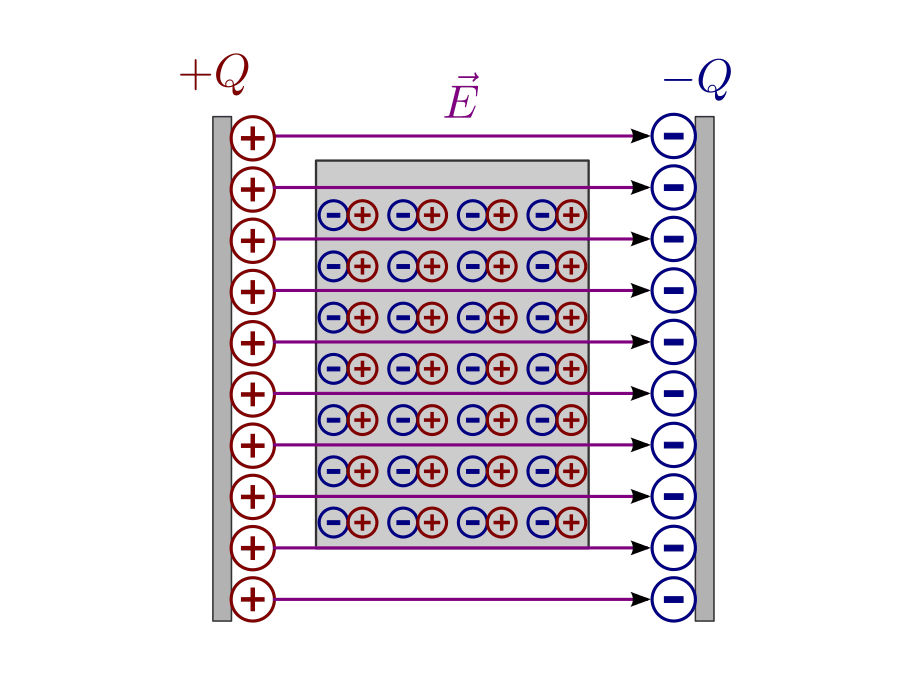
\includegraphics[width=6.2cm]{Bilder/plattenkondensator-polarisation.png}
\end{center}
{\scriptsize Die Moleküle im Dielektrikum richten sich im Feld $\vec E$
aus (\textbf{\emph{Polarisation}}, jeweils als kleiner Dipol $-+$
dargestellt).}

Der Grund: Im Dielektrikum richten sich die Moleküle im elektrischen Feld
aus (Polarisation, siehe Bild). Jedes Molekül wird dabei zu einem kleinen
Dipol mit einer positiven und einer negativen Seite. Im Inneren des
Materials liegt neben der positiven Seite eines Dipols immer die negative
Seite des Nachbardipols, sodass sich diese Ladungen gegenseitig aufheben.

Wie stark ein Material auf diese Weise polarisierbar ist, wird durch die
(dimensionslose) \textbf{\emph{relative Permittivität}} $\varepsilon_r$
beschrieben ($\varepsilon_r>1$ für jedes Material). Beispielsweise hat
Porzellan $\varepsilon_r\approx7$, Wasser (wegen seiner starken
Polarisierbarkeit) sogar $\varepsilon_r\approx80$.

Was an den Rändern des Dielektrikums passiert, und was das für das
Gesamtfeld zwischen den Platten, für die angeschlossene Batterie, für die
Ladung und schliesslich für die Kapazität bedeutet, finden Sie in der
folgenden Herleitung selbst heraus.
\end{theoriebox}

% =============================================================================
% Anwendung: Kapazitive Sensoren
% =============================================================================
\begin{beispielbox}[Anwendung: Kapazitive Sensoren]
Menschliches Gewebe hat wegen seines hohen Wassergehalts eine grosse
relative Permittivität $\varepsilon_r$ (siehe oben) und wirkt deshalb
selbst wie ein Dielektrikum. Nähert sich ein Körperteil einer
Kondensatorplatte, steigt dadurch die gemessene Kapazität messbar an --
genau das nutzen kapazitive Sensoren aus.

\begin{center}
  
\includegraphics[width=5cm]{Bilder/autosensor.png}
  \hspace{0.8cm}
  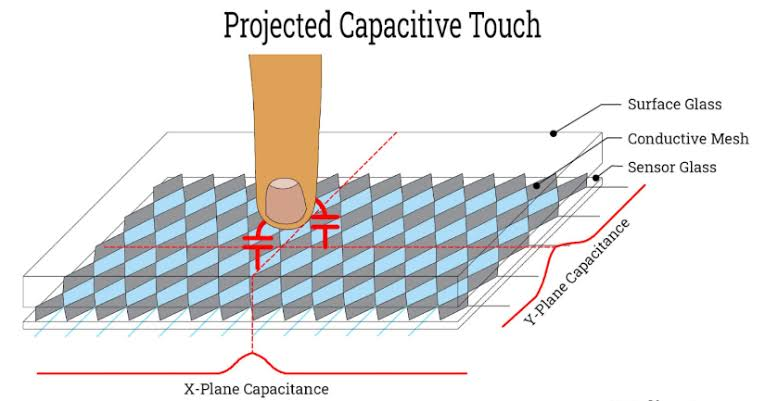
\includegraphics[width=6cm]{Bilder/touchscreen.jpg}
\end{center}
{\scriptsize Links: Kapazitiver Kofferraumsensor -- eine Fussbewegung
unter der Stossstange ändert die Kapazität der Sensorelektrode und löst
das Öffnen aus. Rechts: Prinzip eines kapazitiven Touchscreens -- der
Finger ändert die Kapazität an den Kreuzungen des Elektrodengitters (rote
Kondensatorsymbole), was zeilen- und spaltenweise ausgelesen wird.}

Beim \textbf{\emph{Kofferraumsensor}} mancher Autos genügt eine
Fussbewegung unter der Stossstange, um die Klappe zu öffnen: Der Fuss
verändert die Kapazität einer dort verbauten Elektrode, der Sensor
erkennt die Änderung und löst aus. Der \textbf{\emph{Touchscreen}} Ihres
Smartphones (siehe Einleitung) funktioniert nach demselben Prinzip, nur
mit dem Finger auf einem Gitter aus vielen kleinen Elektroden.
\end{beispielbox}

% =============================================================================
% Herleitung: Kapazität mit Dielektrikum
% =============================================================================
\begin{questions}
\begin{groupbox}[Herleitung (Partnerarbeit): Kapazität mit Dielektrikum]
\question[11] Der Kondensator bleibt während des ganzen Vorgangs an einer
Batterie angeschlossen, die eine \textbf{konstante Spannung $U$} liefert;
der Plattenabstand $d$ bleibt ebenfalls unverändert.
\begin{parts}
  \part[3] Ergänzen Sie das Bild aus der Theorie: Skizzieren Sie den
  Plattenkondensator mit dem polarisierten Dielektrikum, und zeichnen Sie
  ein, wo im Material eine Nettoladung übrig bleibt und weshalb.
  Zeichnen Sie zusätzlich das dadurch entstehende Polarisationsfeld
  $E_{\text{pol}}$ ein.
  \begin{answerbox}
    \rule{0pt}{6.5cm}
  \end{answerbox}
  \begin{solution}
  \begin{center}
    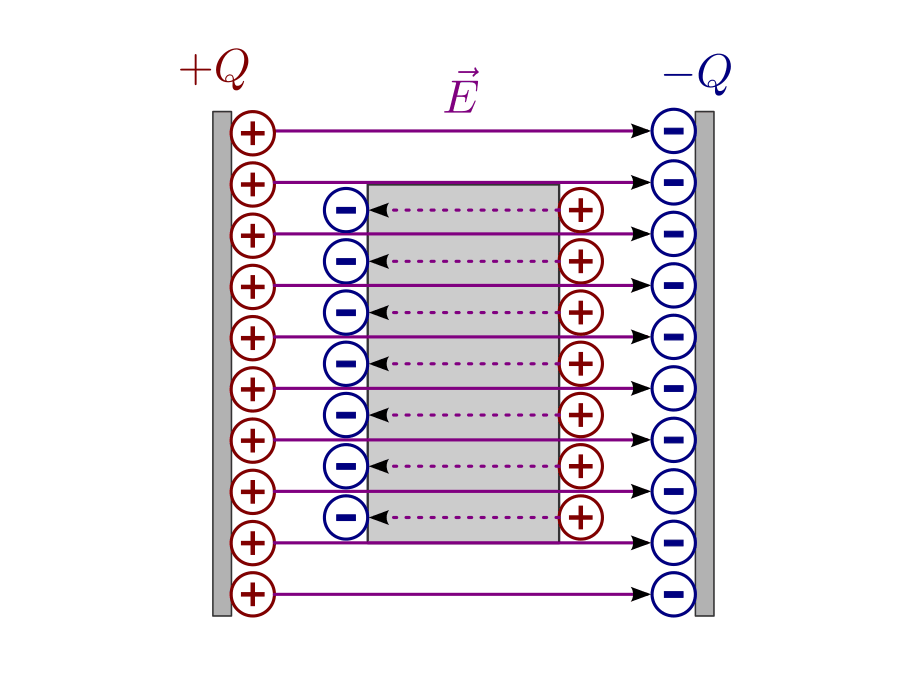
\includegraphics[width=6.2cm]{Bilder/plattenkondensator-influenz.png}
  \end{center}
  Im Inneren des Dielektrikums liegt neben der positiven Seite eines
  Dipols immer die negative Seite des Nachbardipols: Diese Ladungen heben
  sich gegenseitig auf. Nur an den beiden äusseren Rändern des
  Dielektrikums gibt es keinen Nachbardipol zum Ausgleich: Dort bleibt
  eine Nettoladung übrig, negativ auf der Seite der $+Q$-Platte und
  positiv auf der Seite der $-Q$-Platte. Diese Randladung erzeugt das
  eingezeichnete Polarisationsfeld $E_{\text{pol}}$, das dem äusseren
  Feld entgegengerichtet ist.
  \end{solution}

  \part[2] Was bedeutet das für das Gesamtfeld $E$ zwischen den Platten?
  (Tipp: $U=E\cdot d$.)
  \Antwortraum{2}
  \begin{solution}
  Da $U$ und $d$ beide unverändert bleiben, bleibt auch $E=U/d$
  unverändert: Das Gesamtfeld ändert sich nicht.
  \end{solution}

  % Hinweis: Das 4fh-PDF verweist hier (und in der Loesung) auf
  % "Teilaufgabe (a)", gemeint ist inhaltlich (b). Originaltext belassen.
  \part[3] Das Gesamtfeld setzt sich zusammen aus dem Feld der freien
  Ladung, $E_{\text{frei}}=Q/(\varepsilon_0\cdot A)$, und dem
  entgegengerichteten Polarisationsfeld: $E=E_{\text{frei}}-E_{\text{pol}}$.
  Nun ist $E_{\text{pol}}\neq0$ hinzugekommen, während $E$ nach
  Teilaufgabe (a) gleich gross bleiben muss. Was folgt daraus für
  $E_{\text{frei}}$ und damit für die freie Ladung $Q$ auf den Platten? Wie
  reagiert die Batterie darauf?
  \Antwortraum{3}
  \begin{solution}
  $E=E_{\text{frei}}-E_{\text{pol}}$ nach $E_{\text{frei}}$ aufgelöst:
  \[
    E_{\text{frei}} = E + E_{\text{pol}}.
  \]
  Da $E$ nach Teilaufgabe (a) unverändert bleibt und
  $E_{\text{pol}}>0$ neu hinzugekommen ist, muss $E_{\text{frei}}$ grösser
  werden als vorher (als noch $E_{\text{pol}}=0$ war). Mit
  $E_{\text{frei}}=Q/(\varepsilon_0\cdot A)$ aufgelöst nach $Q$:
  \[
    Q = E_{\text{frei}}\cdot\varepsilon_0\cdot A.
  \]
  Da $\varepsilon_0$ und $A$ konstant bleiben, folgt aus grösserem
  $E_{\text{frei}}$ direkt ein grösseres $Q$: Die Batterie pumpt
  zusätzliche freie Ladung auf die Platten, bis sich das ursprüngliche
  Gesamtfeld wieder eingestellt hat.
  \end{solution}

  \part[1] Was folgt daraus für die Kapazität $C=Q/U$?
  \Antwortraum{1}
  \begin{solution}
  Da $Q$ zugenommen hat und $U$ gleich geblieben ist, muss $C=Q/U$
  zunehmen: Die Kapazität steigt.
  \end{solution}

  \part[2] Definiert man die relative Permittivität als das Verhältnis der
  neuen zur ursprünglichen Kapazität, $\varepsilon_r:=C/C_0$, leiten Sie
  damit und mit der bereits bekannten Formel $C_0=\varepsilon_0\cdot A/d$
  (ohne Dielektrikum) die Formel für die Kapazität $C$ mit Dielektrikum
  her.
  \Antwortraum{2}
  \begin{solution}
  \[
    \varepsilon_r = \frac{C}{C_0} \quad\Longrightarrow\quad
    C = \varepsilon_r\cdot C_0 = \varepsilon_r\cdot\varepsilon_0\cdot\frac{A}{d}.
  \]
  \[
    \boxed{C = \varepsilon_r\cdot\varepsilon_0\cdot\frac{A}{d}}
  \]
  \end{solution}
\end{parts}
\end{groupbox}
\end{questions}

\end{document}
